\documentclass[pdf,table]{beamer}
\usepackage{graphicx,hyperref,pdfpages}
\usepackage{tikz}
\usepackage{textpos}
\usepackage{longtable}
\usepackage{listings}
\usepackage{color}
\usepackage{listings}
\usepackage{color}
\usepackage[style=numeric,backend=biber]{biblatex}
%
\usetikzlibrary{arrows}
\usetikzlibrary{positioning,chains,fit,shapes,calc}
\usetikzlibrary{mindmap}
\usetikzlibrary{shapes.multipart}
%
\addbibresource{../CST4025.bib}
\setbeamertemplate{bibliography item}{\insertbiblabel}
%
%defin colours
\definecolor{codegreen}{rgb}{0,0.6,0}
\definecolor{codegray}{rgb}{0.5,0.5,0.5}
\definecolor{codepurple}{rgb}{0.58,0,0.82}
\definecolor{backcolour}{rgb}{0.95,0.95,0.92}
\definecolor{delim}{rgb}{20,105,176}



\lstdefinelanguage{CTO}{
	keywords={abstract, asset, by, concept, default, enum, event, identified, Integer, o, participant, String, transaction },
	comment=[l]{//},
	comment=[s]{/*}{*/},
	string=[b]",
	sensitive=true,
}

\lstdefinelanguage{ACL}{
	keywords={transaction,condition,rule,description,participant,operation,resource,action,ALLOW,READ,ALL,CREATE,UPDATE,DELETE,ANY,DENY},
	comment=[l]{//},
	comment=[s]{/*}{*/},
	string=[b]",
	sensitive=true,
}

%define Javascript language
\lstdefinelanguage{JavaScript}{
keywords={typeof, new, true, false, catch, function, return, null, catch, switch, var, if, in, while, do, else, case, break},
keywordstyle=\color{blue}\bfseries,
ndkeywords={class, export, boolean, throw, implements, import, this},
ndkeywordstyle=\color{darkgray}\bfseries,
identifierstyle=\color{black},
sensitive=false,
comment=[l]{//},
morecomment=[s]{/*}{*/},
commentstyle=\color{purple}\ttfamily,
stringstyle=\color{red}\ttfamily,
morestring=[b]',
morestring=[b]"
}
%define json language
\colorlet{punct}{red!60!black}
\definecolor{background}{HTML}{EEEEEE}
\definecolor{delimiter}{RGB}{20,105,176}
\colorlet{numb}{magenta!60!black}

\lstdefinelanguage{json}{
    numbers=left,
    numberstyle=\scriptsize,
    stepnumber=1,
    numbersep=8pt,
    showstringspaces=false,
    breaklines=true,
    frame=lines,
    backgroundcolor=\color{background},
    literate=
     *{0}{{{\color{numb}0}}}{1}
      {1}{{{\color{numb}1}}}{1}
      {2}{{{\color{numb}2}}}{1}
      {3}{{{\color{numb}3}}}{1}
      {4}{{{\color{numb}4}}}{1}
      {5}{{{\color{numb}5}}}{1}
      {6}{{{\color{numb}6}}}{1}
      {7}{{{\color{numb}7}}}{1}
      {8}{{{\color{numb}8}}}{1}
      {9}{{{\color{numb}9}}}{1}
      {:}{{{\color{punct}{:}}}}{1}
      {,}{{{\color{punct}{,}}}}{1}
      {\{}{{{\color{delimiter}{\{}}}}{1}
      {\}}{{{\color{delimiter}{\}}}}}{1}
      {[}{{{\color{delimiter}{[}}}}{1}
      {]}{{{\color{delimiter}{]}}}}{1},
}
%\lstdefinelanguage{json}{
%    numbers=left,
%    numberstyle=\scriptsize,
%    stepnumber=1,
%    numbersep=8pt,
%    showstringspaces=false,
%    breaklines=true,
%    frame=lines,
%    backgroundcolor=\color{backcolour},
%    literate=
%     *{\{}{{{\color{delim}{\{}}}}{1}
%      {\}}{{{\color{delim}{\}}}}}{1}
%      {[}{{{\color{delim}{[}}}}{1}
%      {]}{{{\color{delim}{]}}}}{1},
%}



\lstdefinestyle{mys}{
	backgroundcolor=\color{backcolour},
	commentstyle=\color{codegreen},
	keywordstyle=\color{magenta},
	stringstyle=\color{codepurple},
	numberstyle=\color{codegray},
	basicstyle=\ttfamily\tiny,
	breakatwhitespace=false,
	breaklines=true
	captionpos=b,
	keepspaces=true,
	numbers=left,
	numbersep=5pt,
	showspaces=false,
	showstringspaces=false,
	showtabs=false,
	tabsize=2}
\lstset{style=mys}



\tikzset{every matrix/.style={ampersand replacement=\&,column sep=1.75cm,row sep=2cm},
		BTWMat/.style={ampersand replacement=\&, column sep=0.75cm,row sep=1cm},
		eulerMat/.style={ampersand replacement=\&,column sep=1.1cm,row sep=2cm},
		vertexHighlight/.style={circle,fill=red!80,inner sep=.1cm,text=white},
		vertex/.style={circle,fill=blue!80,inner sep=.1cm,text=white},
		bank/.style={rectangle,fill=blue!50,inner sep=0.1cm,text=black!80}
		edge/.style={--,line width=2pt},
		Dedge/.style={->,line width=2pt},
		DedgeT/.style={->,line width=1pt},
		BiEdge/.style={<->,line width=2pt},
		BiEdgeT/.style={BiEdge,line width=1pt},
		edgeHighlight/.style={--,line width=2pt,color=red},
		loop/.style={min distance=10mm, line width=2pt},
		loopT/.style={min distance=-10mm, line width=1pt},
		label/.style = { rectangle, rounded corners, draw,
		                 minimum width = 2em, fill = yellow!50,
		                 text = red, font = \tiny\bfseries },
		labelT/.style = { circle, draw, line width=1pt,
		                 minimum width = 1em, fill = yellow!50,
		                 text = red, font = \tiny\bfseries },
		every node/.style={align=center}}



\newcommand{\cwideadline}{3$^{rd}$ November 2019}
\newcommand{\cwiideadline}{5$^{th}$ January 2020}
%\newcommand{\cwiiideadline}{31$^{st}$ March 2017}
%\newcommand{\cwiiideadline}{15$^{th}$ April 2018}
\newcommand{\resitdeadline}{1$^{st}$ August 2020}
\newcommand{\deferraldeadline}{1$^{st}$ August 2020}
\newcommand{\deferraldeadlineMay}{1$^{st}$ May 2020}
\newcommand{\moduleCode}{CST4025}
\newcommand{\moduleLeader}{Dr Ian Mitchell }
\newcommand{\theauthor}{Dr Ian Mitchell }
\newcommand{\academicyear}{2019-20}
\newcommand{\email}{i.mitchell@mdx.ac.uk}
\newcommand{\moduleTitle}{Blockchain Development}
\newcommand{\office}{T108}
\newcommand{\officehours}{Autumn \& Winter Terms: Tuesdays 1515-1615hrs; and, Wednesdays 1415-1515hrs}
\newcommand{\tel}{0208-411-6014}
\newcommand{\deptName}{Computer Science}
%\newcommand{\officehours}{Friday 1100\--1300hrs Autumn Term \\ Thursday 1400\--1600hrs Winter Term}
%\newcommand{\officehours}{Autumn Term: Mondays 1300\--1500hrs \\ Winter Term: Thursdays 1400\--1600hrs

\def\bitcoinA{%
  \leavevmode
  \vtop{\offinterlineskip %\bfseries
    \setbox0=\hbox{B}%
    \setbox2=\hbox to\wd0{\hfil\hskip-.03em
    \vrule height .3ex width .15ex\hskip .08em
    \vrule height .3ex width .15ex\hfil}
    \vbox{\copy2\box0}\box2}}



%
\mode<presentation>{
\usetheme{Madrid}
\usecolortheme{beaver}
}
%
\newcommand{\theweek}{3}
\renewcommand{\theequation}{\theweek.\arabic{equation}}

\title[\moduleCode:L\theweek]{\moduleTitle \\ Week: \theweek \\ Title: Access Control} 
\institute[]{\includegraphics[scale=0.25]{../../../logo/mdxSmall} \\ Middlesex University, \\Dept. of Computer Science, \\London}
\author[\email]{\moduleLeader}
\date{\today}


\begin{document}

\begin{frame}
	\titlepage
\end{frame}

\addtobeamertemplate{frametitle}{}{%
\begin{textblock*}{100mm}(.94\textwidth,-0.85cm)
\includegraphics[scale=0.1]{../../../logo/transparent}
\end{textblock*}}

\begin{frame}{Lecture Aims}
	\begin{block}{Aims}
		Apply and develop Access Control strategies for blockchain.
	\end{block}
\end{frame}

\begin{frame}{Lecture Objectives}
	\begin{block}{Knowledge}
		\begin{itemize}
			\item Implement Blockchain ACL
			\item Role-based access control
			\item Atribute based access control
			\item Apply different strategies of access control
			\item Control the authorisation of Participant's access to assets
		\end{itemize}	
	\end{block}
	\begin{block}{Skills}
		Develop and implement access control for blockchain applications
	\end{block}
\end{frame}


%\begin{frame}{Mandatory Access Control (MAC)}
%	\begin{columns}[T]
%		\begin{column}{0.48\textwidth}
%			\begin{itemize}
%				\item Levels
%			\end{itemize}
%		\end{column}
%		\begin{column}{0.48\textwidth}
%			{\bf MAC}
%		\end{column}
%	\end{columns}	
%\end{frame}

\begin{frame}{Role-Based Access Control (RBAC)}
	\begin{columns}[T]
		\begin{column}{0.48\textwidth}
			\begin{itemize}
				\item Academics, Students, Admin, Management, External 
				\item All have different access to Systems
				\item M:N relationships between users and rights
				\item users cannot pass access permissions on to other users
				\item form of mandatory access control	
				\item not multilevel

			\end{itemize}
		\end{column}
		\begin{column}{0.48\textwidth}
			\begin{block}{RBAC}
				A means of restricting access to objects based on the sensitivity of the information contained within the objects and the formal authorisation of subjects to access information of such sensitivity 
				\cite{ferraiolo2001proposed}
			\end{block}
		\end{column}
	\end{columns}	
\end{frame}


\begin{frame}{RBAC}
	\begin{columns}[T]
		\begin{column}{0.48\textwidth}
			\begin{itemize}
				\item What is a Role?
				\item Set of transactions performed for access
				\item Transactions are allocated roles by SysAdmin
				\item Membership of a role
				\item Academics, Students, Admin, Management, External 
				\item<2-> {\bf Role Explosion}
			\end{itemize}
		\end{column}
		\begin{column}{0.48\textwidth}
			{\bf Exam paper: Do's and Don'ts \cite{mitchell:2019a}}
			\begin{itemize}
				\item<1|only@1> Module Leader writes exam paper.
				\item<1|only@1> Internal moderator reviews exam paper.
				\item<1|only@1> External Examiner checks process
				\item<1|only@1> Module Leader responds
				\item<1|only@1> Administrator signs-off
				\item<1|only@1> Students complete exam
				
				\item<2|only@2> Module leader reviews submitted paper.
				\item<2|only@2> Internal moderator submitting paper.
				\item<2|only@2> External Examiner accessing incorrect papers
				\item<2|only@2> Admin author paper
				\item<2|only@2> Students views paper
			\end{itemize}
		\end{column}
	\end{columns}	
\end{frame}


\begin{frame}{Attribute-Based Access Control}
	\begin{columns}[T]
		\begin{column}{0.48\textwidth}
			\begin{itemize}
				\item Protect objects
				\item Unauthorised operations
				\item ACL \& RBAC %equiv to ABAC
				\item Complex boolean rule set
				\item Rule set evaluates attribute
				\item Extensible Access Control Mark-up Language (XACML)
				\item<3-> \textbf{Attributes}
				\item<3-> \textbf{Subject}
				\item<3-> \textbf{Object}
				\item<3-> \textbf{Operation}
				\item<3-> \textbf{Policy}
				\item<3-> \textbf{Environment}
			\end{itemize}
		\end{column}
		\begin{column}{0.48\textwidth}
			\begin{block}<2->{Definition}
				\begin{quote}
				An access control method where subject requests to perform operations on objects are granted or denied based on assigned attributes of the subject, assigned attributes of the object, environment conditions, and a set of policiesthat are specified in terms of those attributes and conditions.
			\end{quote}
				Vincent C. Hu \textit{et al} \cite{huABAC}
			\end{block}
			\begin{itemize}
				\item 
			\end{itemize}
		\end{column}
	\end{columns}	
\end{frame}


\begin{frame}{Hyperledger - Access Control Language}
	\begin{columns}[T]
		\begin{column}{0.48\textwidth}
			{\bf Review}
			\begin{itemize}
				\item Permissioned blockchain 
				\item Membership Services Provider (MSP)
				\item Fabric Certificate Authority (FCA)
				\item FCA issues Enrollment Certificates (e-certs)
				\item The e-cert is used as a signature
				\item user must register for e-cert
				\item Composer has BNA files
				\item Composer has cards
			\end{itemize}
		\end{column}
		\begin{column}{0.48\textwidth}
			{\bf Attribute-based Access Control (ABAC)}
			\begin{itemize}
					\small
				\item Fabric supports ABAC
				\item access control based on the attributes associated with the user identity
				\item Assets
				\item Participants
				\item Transactions
				\item Events
				\item Business Networks
					\begin{quote}
						A business network is a collection of participants and assets that undergo a life cycle described by transactions. Events occur when transactions complete. 
					\end{quote}
			\end{itemize}
		\end{column}
	\end{columns}	
\end{frame}


\begin{frame}{Access Control Language}{Components}
	\begin{itemize}
		\item Resources
		\begin{itemize}
			\item namespace: org.example.*
			\item namespace(recursive):org.example.** 
			\item Class in a ns: org.example.className 
			\item Instance of a class: org.example.className\#ID
		\end{itemize}
		\item operation
		\item participant
		\item transaction
		\item condition
		\item action
	\end{itemize}
\end{frame}
%	% view https://hyperledger.github.io/composer/v0.19/reference/acl_language.html

\begin{frame}[fragile]{Access Control Language, ACL}{Simple Rules}
	\begin{columns}[T]
		\begin{column}{0.48\textwidth}
			\begin{itemize}
				\item Rules
				\item users
				\item permission
				\item create
				\item read
				\item update
				\item delete
				\item evaluated in order, first rule that matches is executed
		%		\item no matches, then access is denied
			%	\item no rules, no access
			\end{itemize}	
		\end{column}
		\begin{column}{0.48\textwidth}
			{\bf Listing}
			\begin{lstlisting}[language=ACL]
rule {
	description:
	participant:
	operation:
	resource:
	action:
}
			\end{lstlisting}
		\end{column}
	\end{columns}	
\end{frame}

\begin{frame}[fragile]{ACL}{Simple Rules}
			{\bf Listing}
			\begin{lstlisting}[language=ACL, basicstyle=\ttfamily\normalsize]
rule ruleName {
	description:" a brief descript of the rule"
	participant:"namespace.participant"
	operation:
	resource:
	action:
}
			\end{lstlisting}
\end{frame}	

\begin{frame}[fragile]{ACL}
	\textbf{Listing}
			\begin{lstlisting}[language=ACL, basicstyle=\ttfamily\normalsize]
rule ruleName {
	description:" a brief descript of the rule"
	participant:"namespace.participant"
	operation:ALL,CREATE,DELETE,READ,UPDATE
	resource:"namespace.Asset"
	action:ALLOW,DENY
}
		\end{lstlisting}
\end{frame}

\begin{frame}[fragile]{Access Control Language, ACL}{Conditional Rules}
	\begin{columns}[T]
		\begin{column}{0.48\textwidth}
			\begin{itemize}
				\item Rules
				\item Trader example
				\item trader 1: current owner / seller
				\item trader 2: new owner / buyer
				\item only an owner of an asset should be able to sell it
			\end{itemize}	
		\end{column}
		\begin{column}{0.48\textwidth}
			{\bf Listing}
			\begin{lstlisting}[language=ACL]
rule ownerOnlyAccess{
	description: "Owners get full access and the right to sell"
	participant(p): "org.example.trading.Trader"
	operation: ALL
	resource(r): "org.example.trading.Commodity"
	condition: (p==r.owner)
	action:ALLOW
 }
			\end{lstlisting}
		\end{column}
	\end{columns}	
\end{frame}



\begin{frame}{Case Study - Trader Network}
	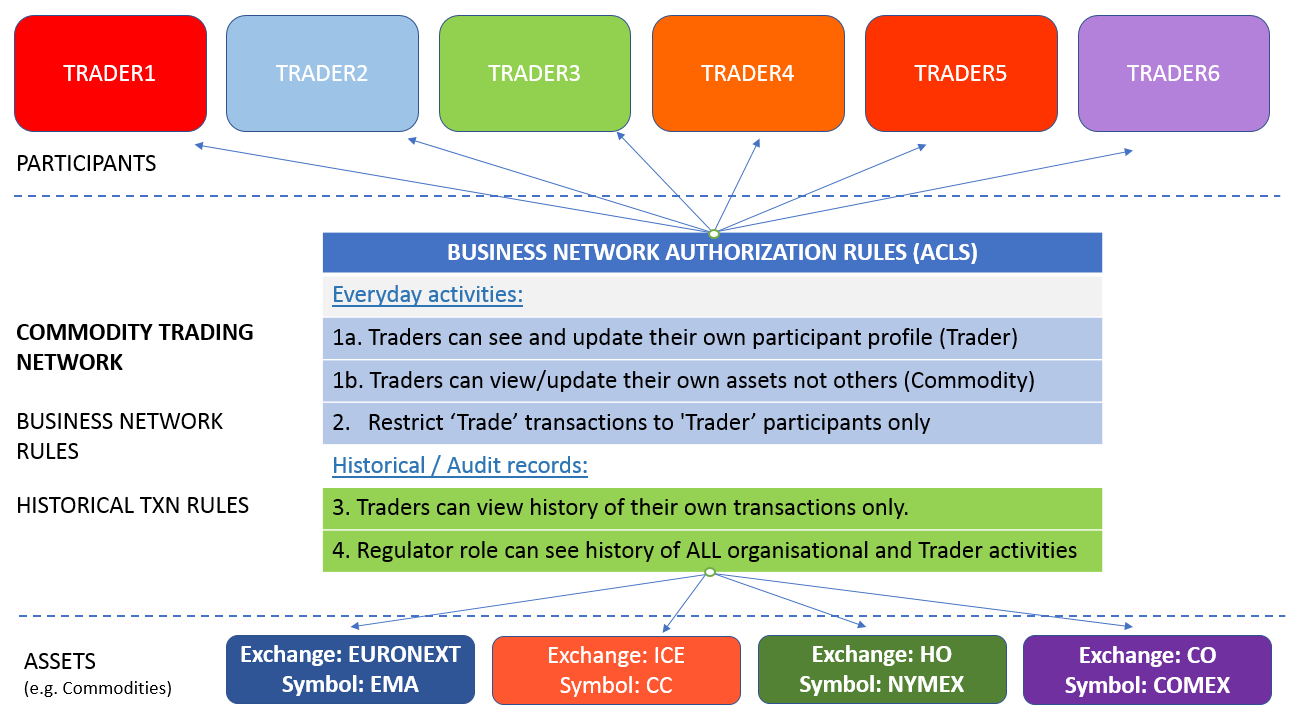
\includegraphics[scale=0.3]{trader}
\end{frame}

\begin{frame}[fragile]{Rule Implementation}{Trader Network}
	\begin{columns}[T]
		\begin{column}{0.48\textwidth}
			\begin{itemize}
				\item Rules are generic and allow all access
				\item Add 6 traders to the network
				\item Add more commodities to the network
				\item Look at rules
				\item Remove this rule
				\item keep the admin rules (on next slide)
			\end{itemize}	
		\end{column}
		\begin{column}{0.48\textwidth}
			{\bf Listing}
			\lstinputlisting[language=ACL,firstline=17, lastline=23, firstnumber=17]{trader-/permissions.acl}
		\end{column}
	\end{columns}	
\end{frame}

\begin{frame}[fragile,allowframebreaks]{Trader Network}{Permissions.acl}
	\lstinputlisting[language=ACL,firstline=24,firstnumber=24]{trader-/permissions.acl}
\end{frame}

\begin{frame}[fragile]{Rule}{Traders can only see themselves}
	\begin{columns}[T]
		\begin{column}{0.48\textwidth}
			\begin{itemize}
				\item If we have six traders, should traders be able to see each other?
				\item So here is a rule that allows traders to see themselves only
				\item This is a condition.
				\item The solution slightly abuses the resource
				\item A resource does not have to be an asset, it can also be a participant
				\item Condition is when the identifiers are equal allow updates and reads
			\end{itemize}
		\end{column}
		\begin{column}{0.48\textwidth}
			\begin{lstlisting}[language=ACL]
rule traderSeeThemselvesOnly{
	description: "Trader can only see themselves"
	participant(p):"org.example.trader.Trader"
	operation: READ, UPDATE
	resource(r): "org.example.trader.Trader"
	condition: (p.getIdentifier() == r.getIdentifier())
	action: ALLOW
	}
			\end{lstlisting}
		\end{column}
	\end{columns}	
\end{frame}

\begin{frame}[fragile]{Rule}{Traders can only trade assets they own}
	\begin{columns}[T]
		\begin{column}{0.48\textwidth}
			\begin{itemize}
				\item You should not be able to trade something you don't own
				\item rule is to allow traders to only sell assets they own
				\item This is a more traditional condition
				\item participant: trader
				\item resource: commodity (asset)
				\item condition: traderID == owner ID
			\end{itemize}
		\end{column}
		\begin{column}{0.48\textwidth}
			\begin{lstlisting}[language=ACL]
rule traderUpdateReadTheirCommodities{
	description: "trader can see/sell/update their own commodities"
	participant(p): "org.example.trader.Trader"
	operation: ALL
	resource(r): "org.example.trader.Commodity"
	condition: (p.getIdentifier()==r.owner.getIdentifier())
	action: ALLOW 
}	
			\end{lstlisting}
		\end{column}
	\end{columns}	
\end{frame}

\begin{frame}[fragile]{Rule}{Traders To Submit Transactions}
	\begin{columns}[T]
		\begin{column}{0.48\textwidth}
			\begin{itemize}
				\item allow access to transaction, trade
				\item participant: trader
				\item resource: trade (transaction)
				\item condition: none
				\item action: allow
				\item operation: all
			\end{itemize}
		\end{column}
		\begin{column}{0.48\textwidth}
			\begin{lstlisting}[language=ACL]
rule traderToSubmitTX{
	description:"Enable Traders to trade, submit transactions"
	participant:"org.example.trader.Trader"
	operation:ALL
	resource:"org.example.trader.Trade"
	action: ALLOW
	}
			\end{lstlisting}
		\end{column}
	\end{columns}	
\end{frame}



%\begin{frame}{Case Study - Line of Credit}
%
%\end{frame}


\begin{frame}{Summary}
	\begin{itemize}
		\item Top-to-bottom evaluation
		\item most specific to least specific
		\item As soon as participant, operation and resource match then subsequent rules are not executed
		\item If no ACL rule fires then AC is denied
	\end{itemize}
\end{frame}

\begin{frame}[allowframebreaks]{References}

\printbibliography
	
\end{frame}
	
\begin{frame}
	\frametitle{Web Resources}
	\begin{itemize}
	\item \url{http://hyperledger.org}
	\end{itemize}
\end{frame}

%\begin{frame}[fragile]{Enumerator Types}
%	\begin{columns}[T]
%		\begin{column}{0.48\textwidth}
%			\begin{itemize}
%				\item XXX 
%			\end{itemize}
%		\end{column}
%		\begin{column}{0.48\textwidth}
%			{\bf XXX}
%			\begin{lstlisting}
%			\end{lstlisting}
%		\end{column}
%	\end{columns}	
%\end{frame}
%
%

%\begin{frame}{X}
%	\begin{columns}[T]
%		\begin{column}{0.48\textwidth}
%			\begin{itemize}
%				\item XXX 
%			\end{itemize}
%		\end{column}
%		\begin{column}{0.48\textwidth}
%			{\bf XXX}
%		\end{column}
%	\end{columns}	
%\end{frame}


\end{document}
